\section{Installation der elektrischen Komponenten}
Die elektrische Installation basiert auf der Versorgungsspannung von 5 V.  
Alle LED-Streifen sowie der Mikrocontroller werden damit versorgt und haben einen gemeinsamen Ground.  

Es werden drei LED-Streifen eingesetzt. 
Der erste hat 256 \gls{ws2812b}-\gls{led}s und wird für die Anzeige von Stunden und Minuten, der Außentempreatur und dem Wetter verwendet.  
Der zweite hat 60 \gls{ws2812b}-\gls{led}s und wird für die Sekundenanzeige genutzt.
Der dritte hat 37 \gls{ws2812b}-\gls{led}s und wird für die Anzeige der Zusatzfunktionen genutzt.
Die Datenleitungen der LED-Streifen werden jeweils auf separate GPIO-Pins des Mikrocontrollers geführt.  

Die Dimensionierung des Netzteils erfolgt auf Basis der maximal möglichen Leistungsaufnahme.  
Die Gesamtleistung ergibt sich aus der maximalen Anzahl an LEDs die gleichzeitig aktiv sein können und deren spezifischer Leistungsaufnahme.  
Für die Berechnung kann folgende Beziehung verwendet werden:  
\[
P_{\text{gesamt}} = N_{\text{LED}} \cdot P_{\text{LED}}
\]

Die Leistungsaufnahme pro LED kann über die Streckenleistung bestimmt werden welche im Datenblatt der verwendeten \gls{led}-Streifen angegeben ist:  
\[
P_{\text{LED}} = \frac{P_{\text{pro Meter}}}{N_{\text{LED pro Meter}}}
\]

Für den verwendeten LED-Streifen ergeben sich laut Herstellerangaben eine Leistungsaufnahme von  
\[
P_{\text{pro Meter}} = 6\,\text{W/m}
\]
bei einer Bestückung von  
\[
N_{\text{LED pro Meter}} = 30\,\text{LED/m}
\]

Damit ergibt sich die Leistungsaufnahme einer einzelnen LED zu:  
\[
P_{\text{LED}} = \frac{6\,\text{W/m}}{30\,\text{LED/m}}
= 0{,}2\,\text{W}
\]

Im ungünstigsten Fall sind während des Boot-Modus kurzzeitig alle 256 LEDs des Hauptstreifens, bei voller Helligkeit, gleichzeitig aktiv. Daraus ergibt sich die maximale Gesamtleistung zu:  
\[
P_{\text{gesamt}} = 256 \cdot 0{,}2\,\text{W}
= 51{,}2\,\text{W}
\]

Die Stromaufnahme berechnet sich mit:  
\[
I_{\text{gesamt}} = \frac{P_{\text{gesamt}}}{U}
\]

Bei einer Versorgungsspannung von  
\[
U = 5\,\text{V}
\]
ergibt sich:  
\[
I_{\text{gesamt}} = \frac{51{,}2\,\text{W}}{5\,\text{V}}
= 10{,}24\,\text{A}
\]

Die mindestens erforderliche Netzteilleistung ergibt sich anschließend zu:  
\[
P_{\text{Netzteil}} = U \cdot I_{\text{gesamt}}
\]

Somit ergibt sich eine erforderliche Mindestleistung von:  
\[
P_{\text{Netzteil}} = 5\,\text{V} \cdot 10{,}24\,\text{A}
= 51{,}2\,\text{W}
\]

Obwohl im Boot-Modus kurzzeitig alle 256 LEDs des Hauptstreifens bei voller Helligkeit aktiviert werden, tritt dieser Zustand nur für etwa eine Sekunde auf. 
Für die thermische und dauerhafte Auslegung des Netzteils ist dieser kurzzeitige Spitzenwert nicht maßgebend.
Im normalen Betrieb sind deutlich weniger LEDs gleichzeitig aktiv. 
Der kurzzeitige Einschaltzustand während des Boot-Modus kann vom Netzteil als kurzzeitige Lastspitze bereitgestellt werden. 
Aus diesem Grund wird ein Netzteil mit einer Ausgangsstromstärke von \SI{10}{\ampere} bei \SI{5}{\volt} verwendet.
Mit diesem ist auch die Leistungsaufnahme des \gls{esp32c6} und des \gls{dht22} Sensors mit genügend Reserve abgedeckt.

In Abbildung~\ref{fig:Schaltplan} ist noch der Schaltplan der Wortuhr dargestellt.
\todo{Schaltplan}
\begin{figure}[H]
	\centering
	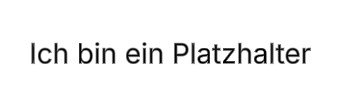
\includegraphics[width=0.3\linewidth]{inhalt/bilder/Platzhalter.jpg}
	\caption{Dargestelt ist der Schaltplan der Wortuhr mit allen angeschlossenen Komponenten und Pinbelegung des ESP32-C6.}
	\label{fig:Schaltplan}
\end{figure}